\chapter{Memorial descritivo}

\section*{Conteúdo e acessórios}

\begin{table}[H]
\centering
\begin{tabular}{|l|l|l|}
\hline
Equipamento & Descrição  & Quantidade \\ \hline
Maleta de controle & Estrutura que comporta a interface de usuário & 1 \\ \hline
Maleta de suporte & Estrutura que armazena, transporta e alimenta os & \\ & equipamentos de abastecimento e ignição  & 1 \\ \hline
Adaptador dos & Sistema de acoplamento entre válvula e motor & \\ atuadores & & 2 \\ \hline
Mangueira & Mangueira de conexão entre adaptador e válvula anti-retorto & 1 \\ \hline
Válvula anti-retorno & Válvula que garante o transporto hidráulico em uma & \\ & única direção & 1 \\ \hline
Engate rápido & Conector com a parte interna do foguete & 1 \\ \hline
Carregador & Estrutura de carregamento das baterias & 1 \\ \hline
Módulo base de & Estrutura que controla os sensores da base de lançamento & \\ lançamento & e os atuadores do abastecimento & 1 \\ \hline
\end{tabular}
\end{table}

\section*{Maleta de controle}

\subsection*{Características}

\begin{figure}[H]
  \centering
  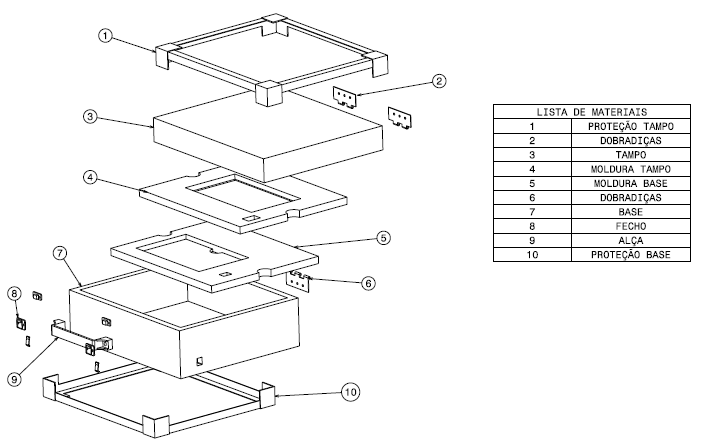
\includegraphics[scale=0.7]{Figuras/gcs_explode.png}
  \caption{Layout da Maleta de Controle - Estrutura}
  \label{fig:gcs_explode}
\end{figure}

\begin{figure}[H]
  \centering
  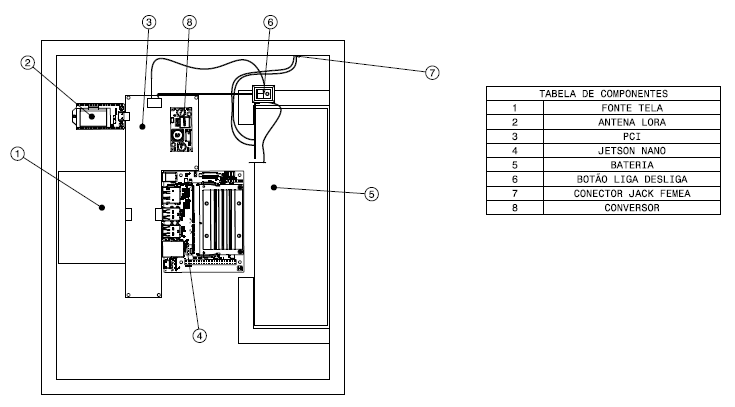
\includegraphics[scale=0.7]{Figuras/gcs_componentes.png}
  \caption{Layout da Maleta de Controle - Componentes}
  \label{fig:gcs_explode}
\end{figure}

\subsection*{Informações técnicas}

\begin{table}[H]
\centering
\begin{tabular}{|l|l|}
\hline
Modelo & RGS2020A-GCS \\ \hline
Tensão & 12V \\ \hline
%Frequência &  \\ \hline
Potência & 97 Wh \\ \hline
Dimensões & 352x300x152(mm) \\ \hline
Peso & 5 kg \\ \hline
Tamanho da tela & 9' \\ \hline
\end{tabular}
\end{table}

\subsection*{Instruções de uso}

\par Coloque a maleta sobre uma superfície nivelada, abra os fechos da maleta, indicados na imagem e depois aperte o botão de ligar/desligar para iniciar a missão.

\section*{Maleta de suporte}

\subsection*{Características}

\begin{figure}[H]
  \centering
  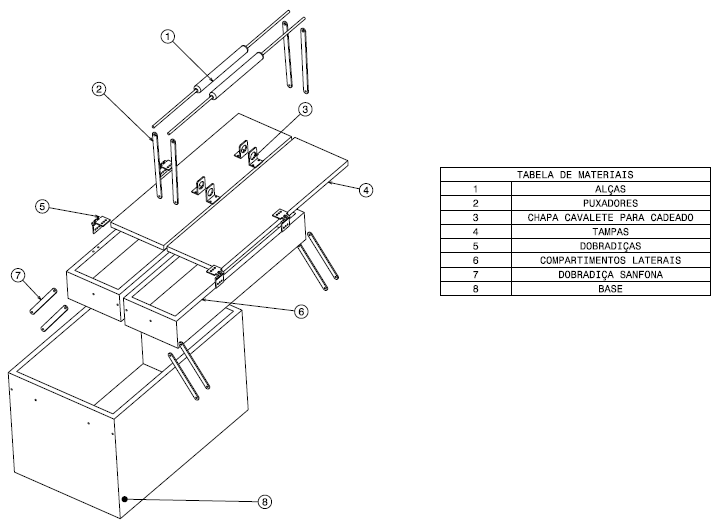
\includegraphics[scale=0.8]{Figuras/suporte_explode.png}
  \caption{Layout da Maleta de Suporte}
  \label{fig:suporte_explode}
\end{figure}

\subsection*{Informações técnicas}

\begin{table}[H]
\centering
\begin{tabular}{|l|l|}
\hline
Modelo & RGS2020A-Suporte \\ \hline
Tensão & 12V \\ \hline
%Frequência &  \\ \hline
Potência & 40 Wh \\ \hline
Dimensões & 520x330x568 (mm)\\ \hline
Peso & 10 kg \\ \hline
\end{tabular}
\end{table}

\subsection*{Instruções de uso}

\par Primeiro coloque as alças laterais para baixo, depois abra os cadeados e os retire dos cavaletes. Puxe as tampas para cima e abra os compartimentos superiores lateralmente. Retire os equipamentos removíveis da maleta, e monte-os de forma adequada. Por fim conecte os cabos de energia no local indicado para a alimentação do sistema dentro da maleta.

\section*{Carregador}

\subsection*{Características}

\begin{figure}[H]
  \centering
  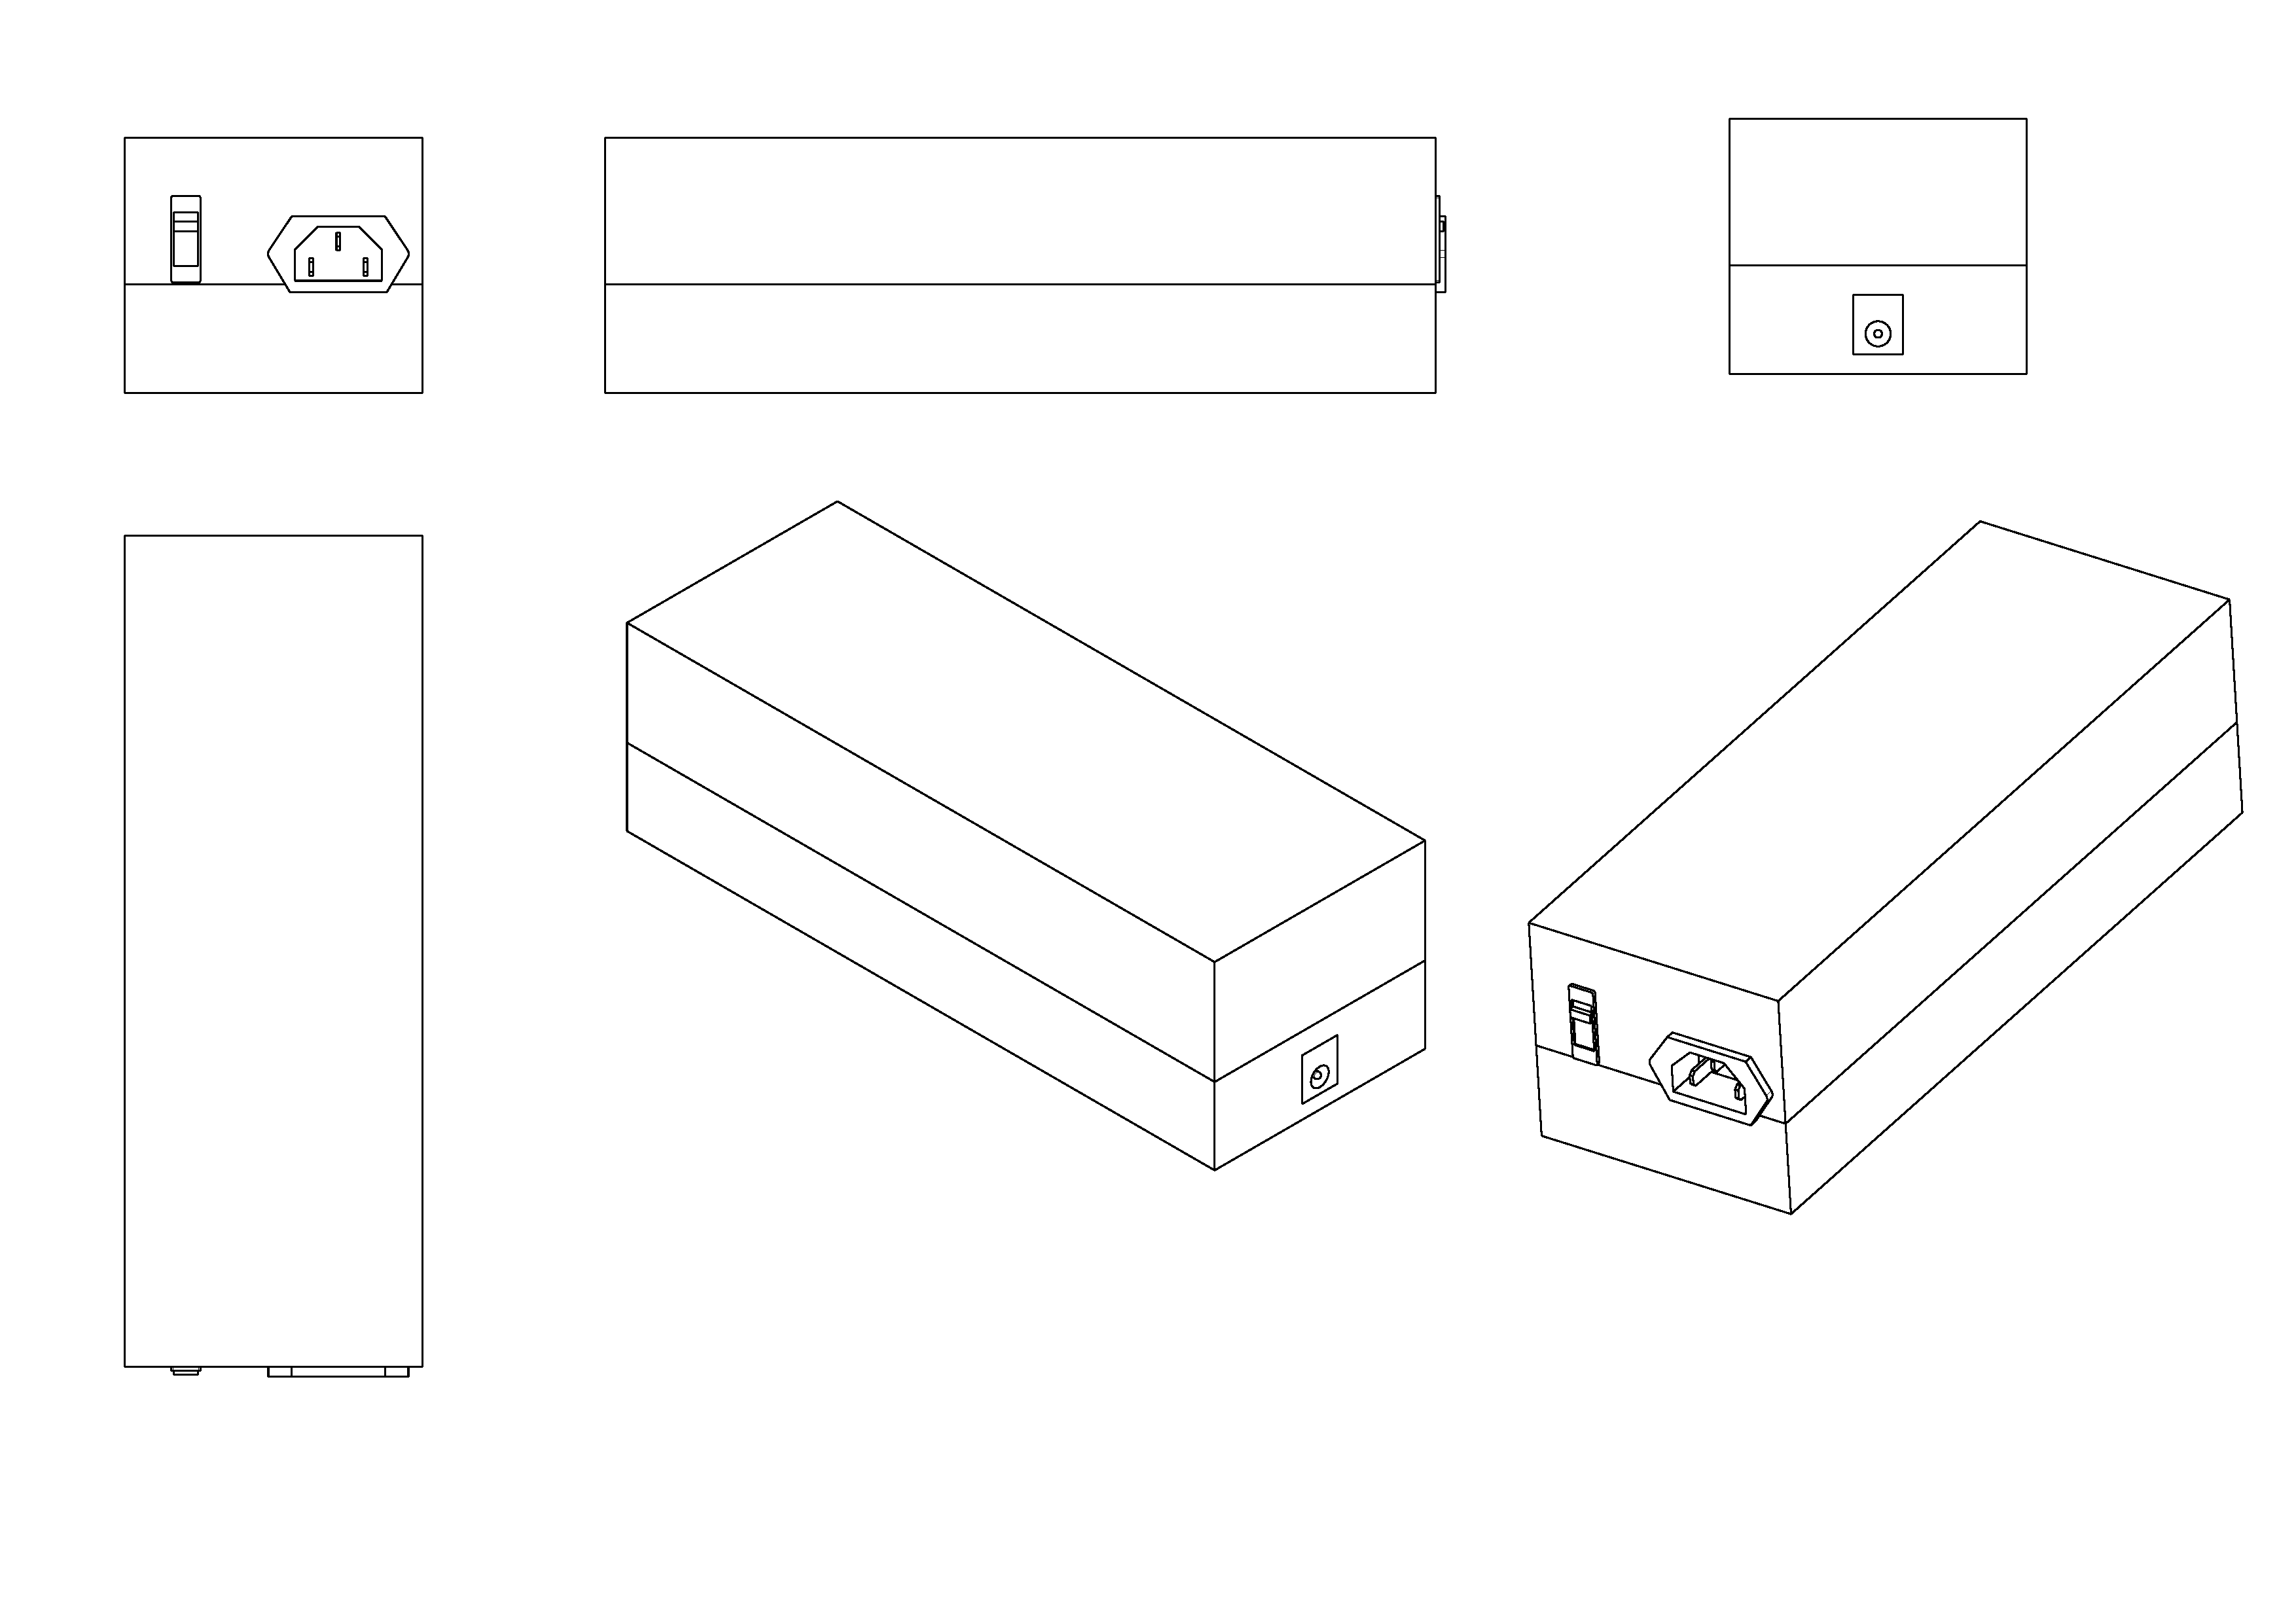
\includegraphics[scale=0.2]{Figuras/Vistas_carregador.pdf}
  \caption{Layout do Carregador}
  \label{fig:suporte_explode}
\end{figure}

\section*{Controlador da Base de lançamento}

\subsection*{Características}

\begin{figure}[H]
  \centering
  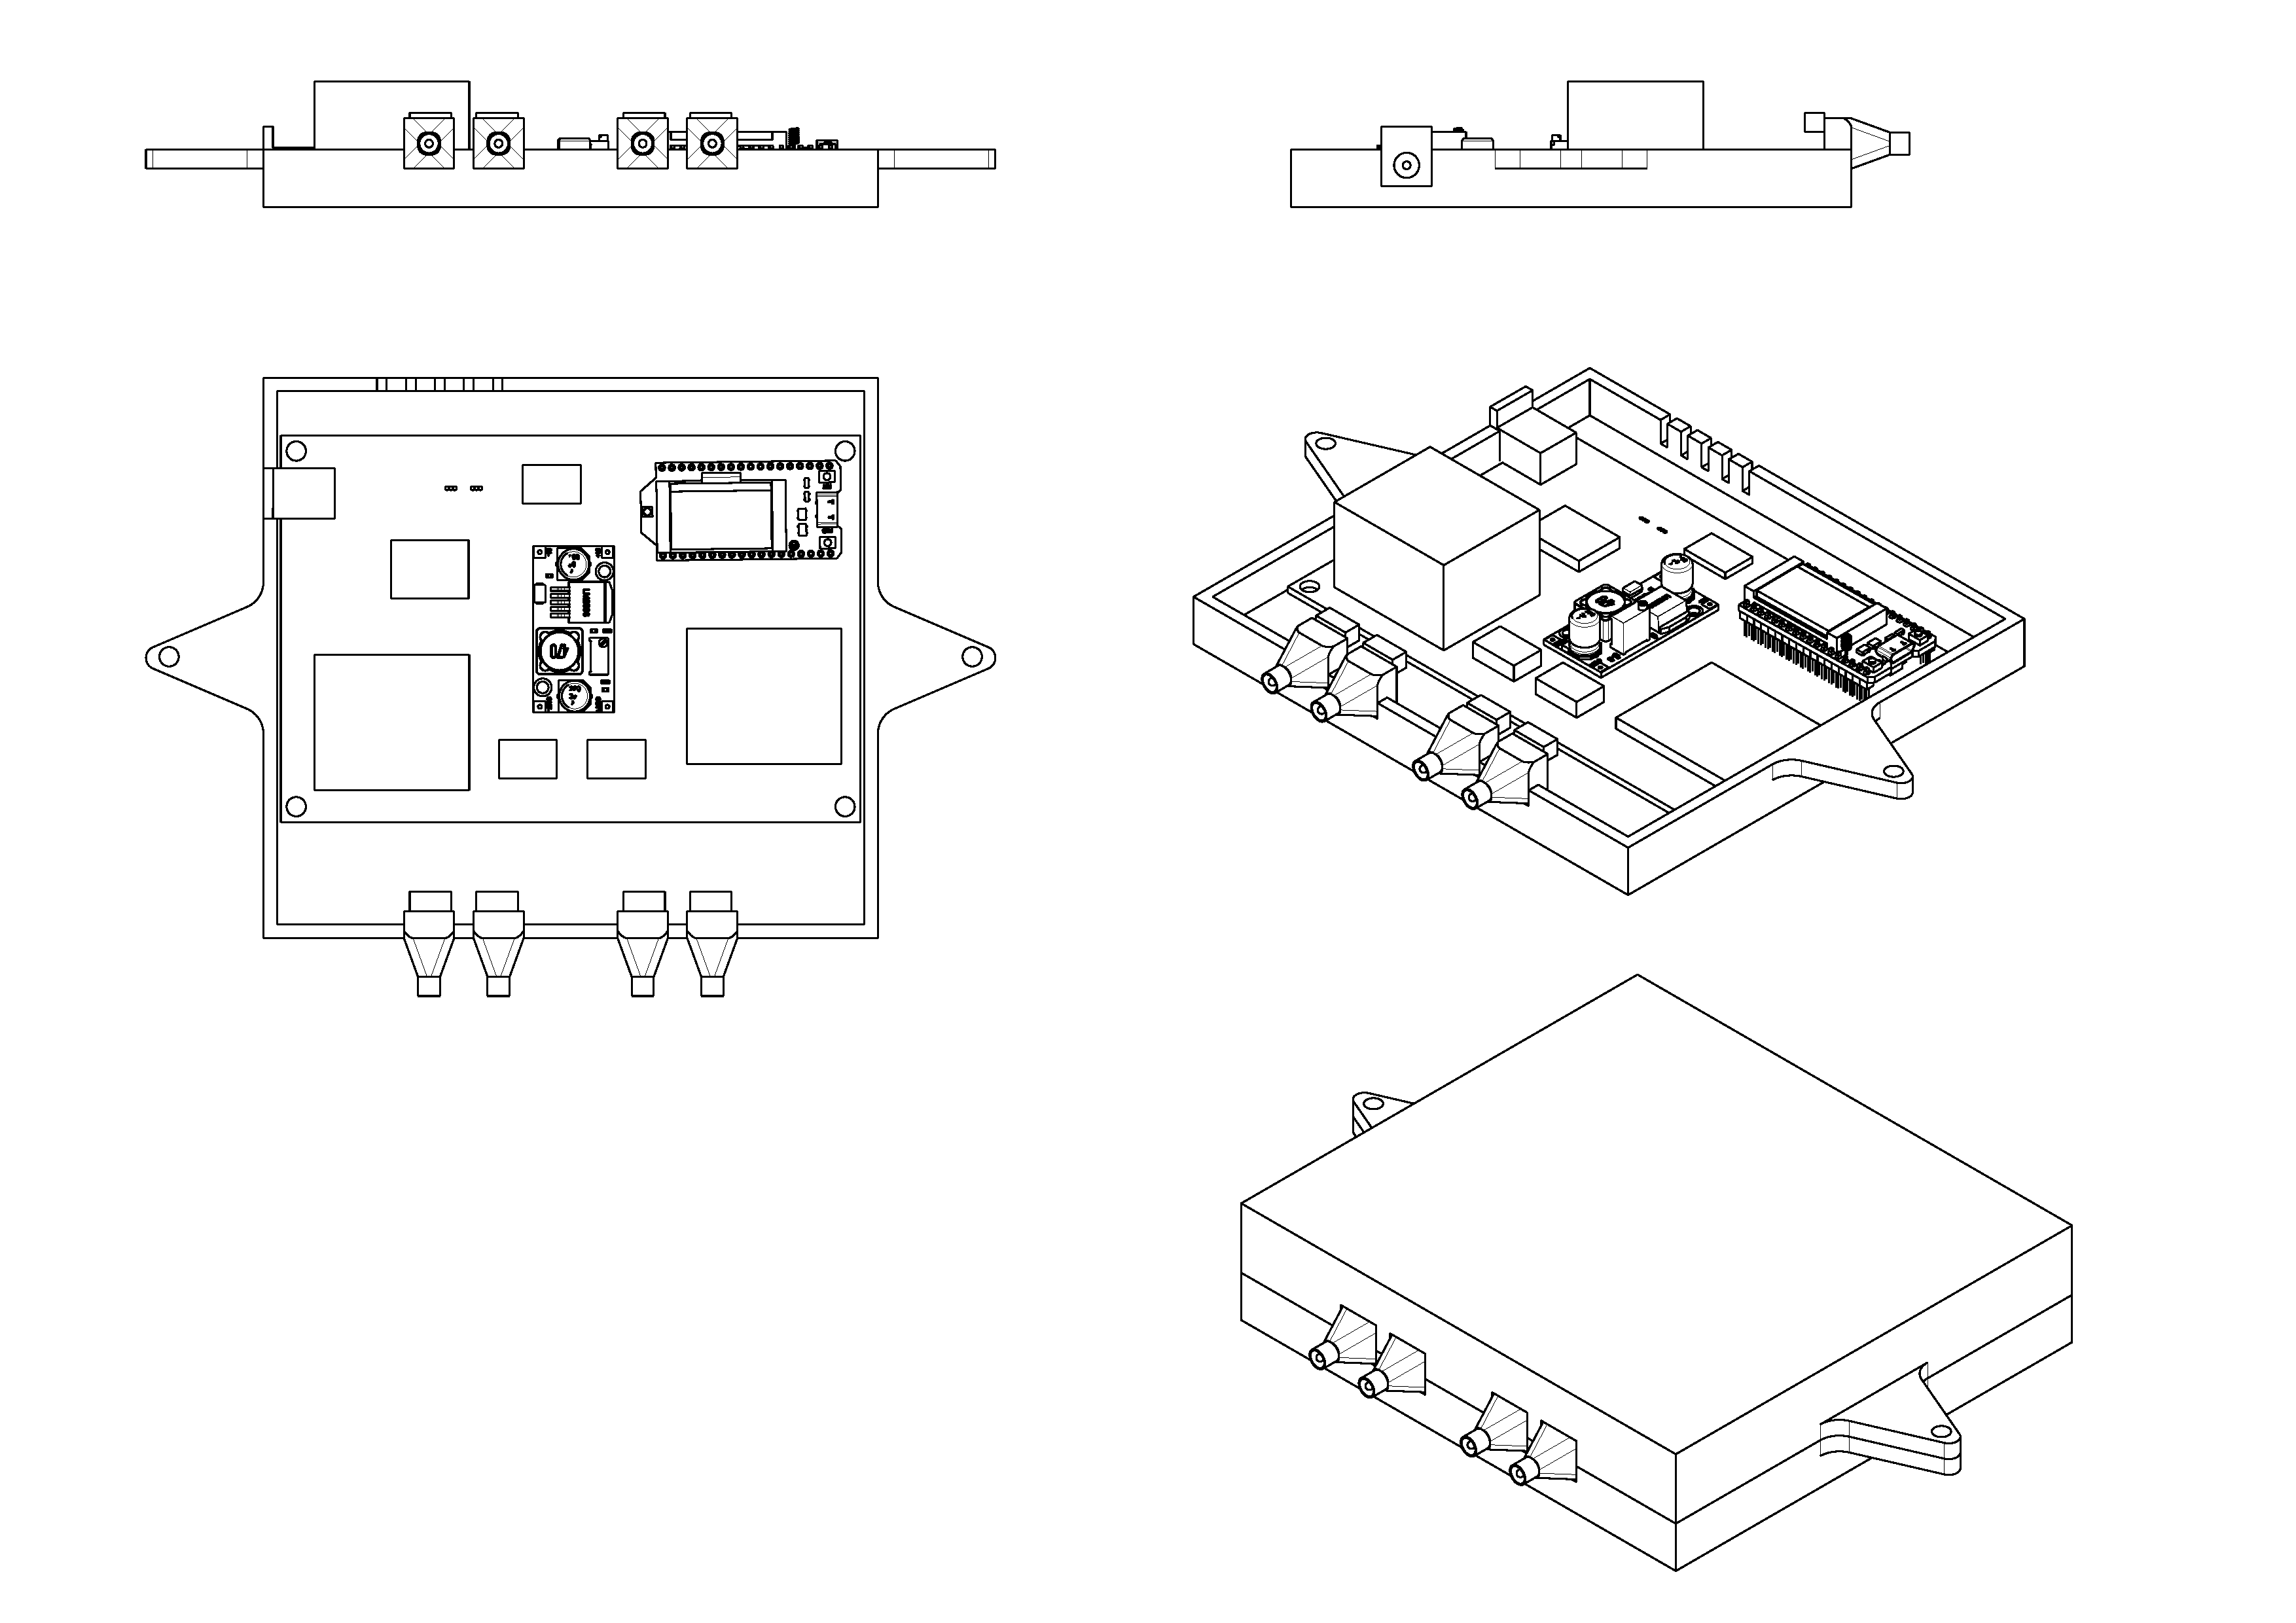
\includegraphics[scale=0.2]{Figuras/Vistas_caseelet.pdf}
  \caption{Layout do Controlador da Base de lançamento}
  \label{fig:suporte_explode}
\end{figure}

%\section*{Abastecimento}

%\subsection*{Características}

%\subsection*{Informações técnicas}

%\subsection*{Instruções de uso}

\section*{Dentro do Foguete}
\subsection*{Características}
\par Como o foguete é  uma caixa preta no projeto foi projetado um circuito completo e adaptável para ser adicionado dentro do foguete em uma PCI mostrada na figura \ref{fig:Dimensões da PCI do f} com as dimensões mostradas e com a opção de fixação dentro do foguete por parafusos de rosca m5.

\begin{figure}[H]
  \centering
  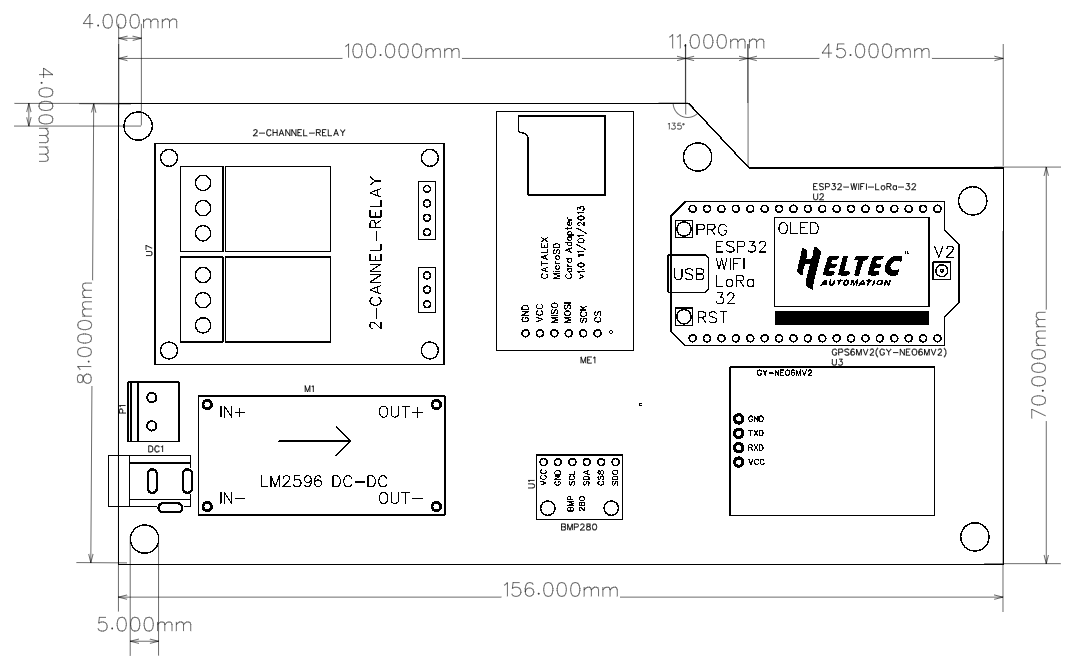
\includegraphics[scale=0.3]{Figuras/PCB_PCB_interna do foguete.png}
  \caption{Dimensões da PCI do foguete.}
  \label{fig:Dimensões da PCI do f}
\end{figure}

\subsection*{Informações técnicas}
\par A placa de circuito impresso do foguete foi projetada de forma a ser funcional e pequena para melhor acomodação dentro do foguete, há cinco furos para a fixação da mesma no foguete todas com rosca M5 possui demissões de 156.0 x 81.0 mm espessura de 1.6mm e espessura de cobre de 1$oz$.

\subsection*{Instruções de uso}

\par Para a utilização do circuito do foguete inicialmente é necessário a gravação da ESP 32 LoRa com auxílio de um cabo Micro-USB e um computador pessoal.Para isso é necessário ter a IDE do Arduíno instalado no computador pessoal, pode ser obtida através do link : https://www.arduino.cc/en/software e siga os passos abaixo:
\begin{itemize}
    \item Apos entrar no site clique no local indicado na figura \ref{fig:Download ide} e faça o download para a versão do seu sistema operacional;
    \begin{figure}[H]
  \centering
  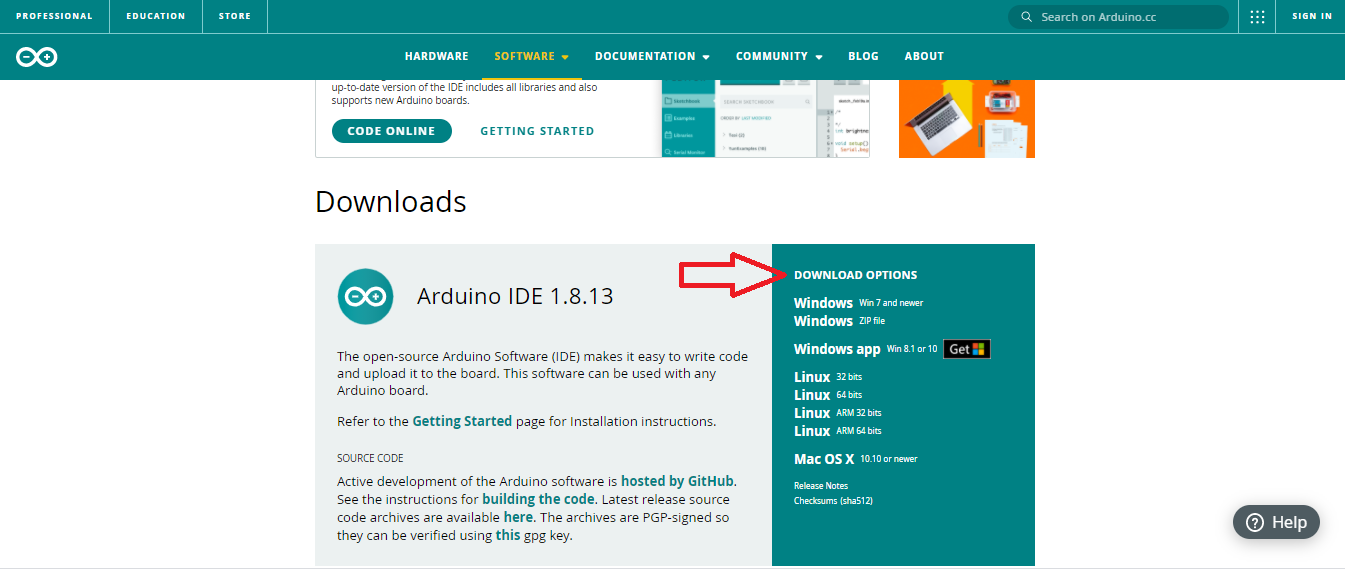
\includegraphics[scale=0.4]{Figuras/passo1.png}
  \caption{Passo 1 - Download IDE}
  \label{fig:Download ide}
\end{figure}
\item Apos o download basta instalar o programa.
\item Clique na aba Arquivos e em seguida em preferências;
   \begin{figure}[H]
  \centering
  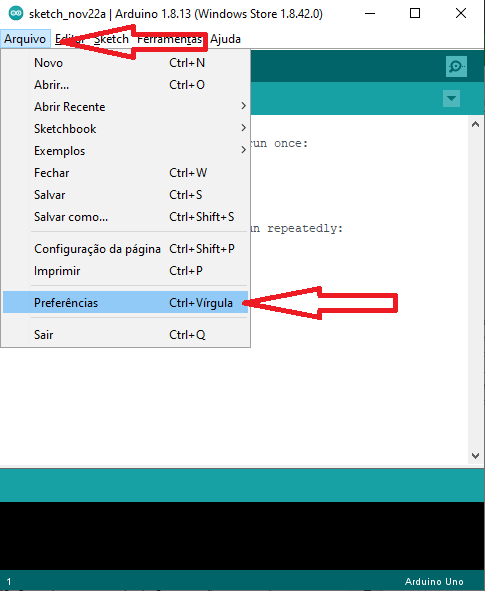
\includegraphics[scale=0.4]{Figuras/passo2.png}
  \caption{Passo 2}
  \label{fig:Download ide}
\end{figure}

\item Adicione a URL para instalação do pacote da ESP32 \\https://dl.espressif.com/dl/package_esp32_index.json

   \begin{figure}[H]
  \centering
  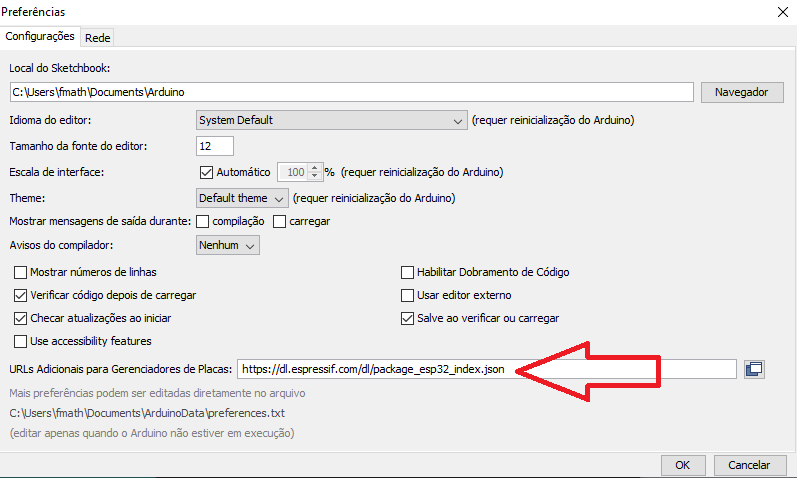
\includegraphics[scale=0.4]{Figuras/passo3.png}
  \caption{Passo 3}
  \label{fig:Download ide}
\end{figure}

\item Vá no ícone \textbf{ Ferramentas/Placa:"Arduino Uno"/gerenciador de Placas...}

   \begin{figure}[H]
  \centering
  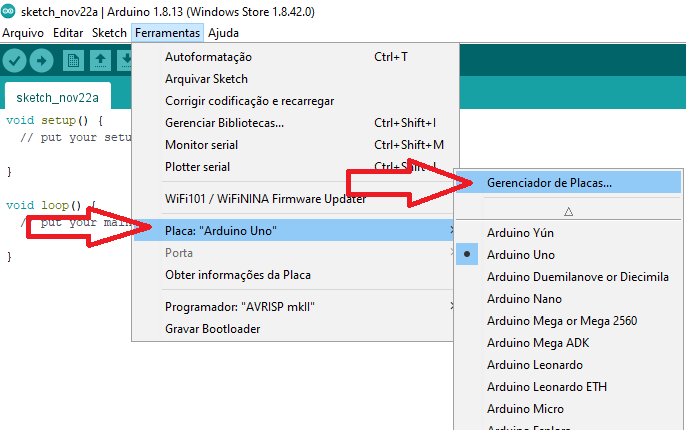
\includegraphics[scale=0.4]{Figuras/passo4.png}
  \caption{Passo 4}
  \label{fig:Download ide}
\end{figure}
\item Pesquise por ESP32 na aba de pesquisa e clique em instalar nos arquivos da ESP32.
   \begin{figure}[H]
  \centering
  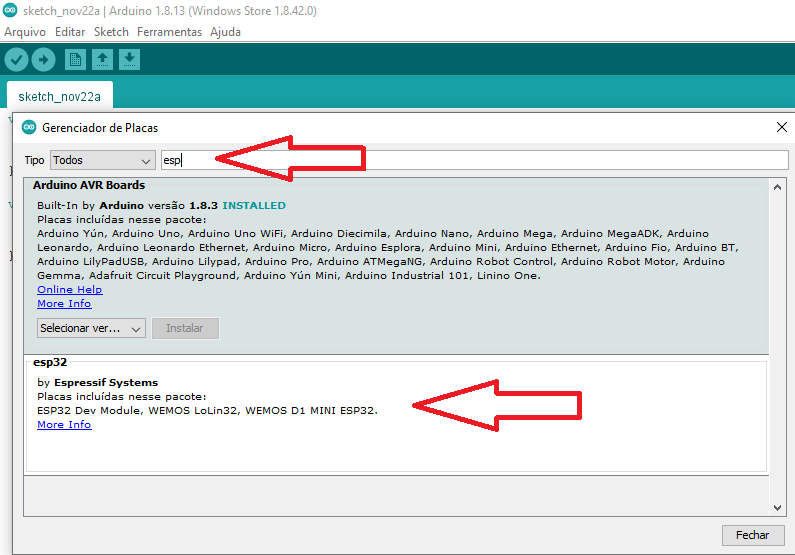
\includegraphics[scale=0.4]{Figuras/passo5.png}
  \caption{Passo 5}
  \label{fig:Download ide}
\end{figure}
\item Vá no ícone\textbf{ Sketch/Inclui Biblioteca/Gerenciador de Bibliotecas...}
   \begin{figure}[H]
  \centering
  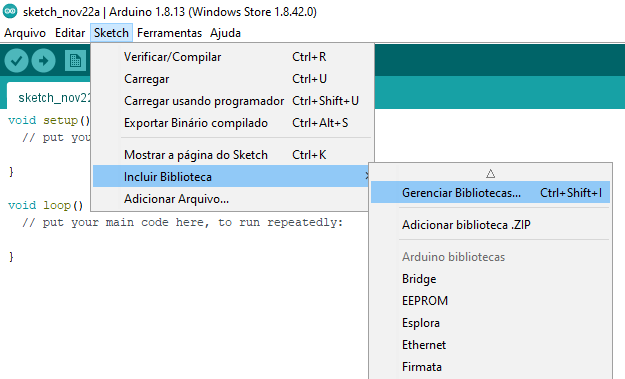
\includegraphics[scale=0.4]{Figuras/passo6.png}
  \caption{Passo 6}
  \label{fig:Download ide}
\end{figure}
\item Pesquise por HELTEC na aba de pesquisa e clique em instalar .
   \begin{figure}[H]
  \centering
  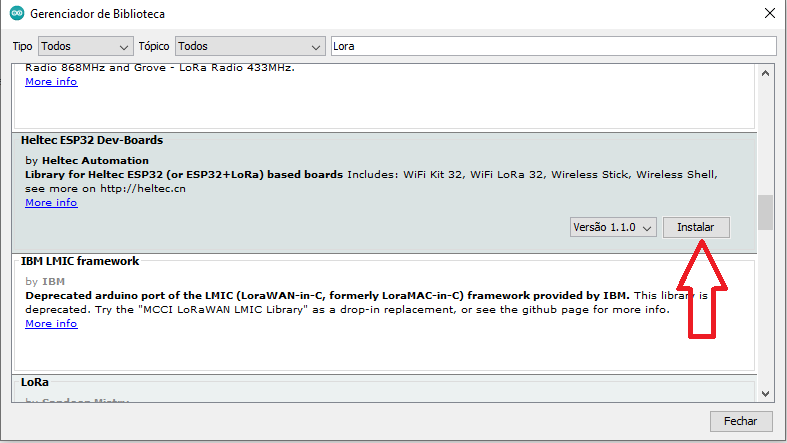
\includegraphics[scale=0.4]{Figuras/passo7.png}
  \caption{Passo 7}
  \label{fig:Download ide}
\end{figure}
\item Pesquise por LoRa na aba de pesquisa e clique em instalar .
   \begin{figure}[H]
  \centering
  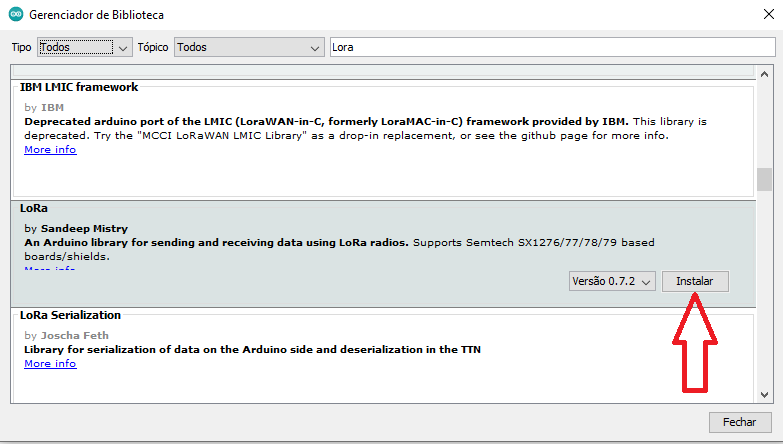
\includegraphics[scale=0.4]{Figuras/passo8.png}
  \caption{Passo 8}
  \label{fig:Download ide}
\end{figure}

\item Apos a instalação do programa e bibliotecas necessárias basta utilizar um cabo Micro-USB\ref{fig:Cabo MicroUSB}  conectado a ESP32 LoRa da Heltech e a um computador pessoal que esteja com as etapas acima feitas e instalar o código disponibilizado para o funcionamento do hardware em questão.
   \begin{figure}[H]
  \centering
  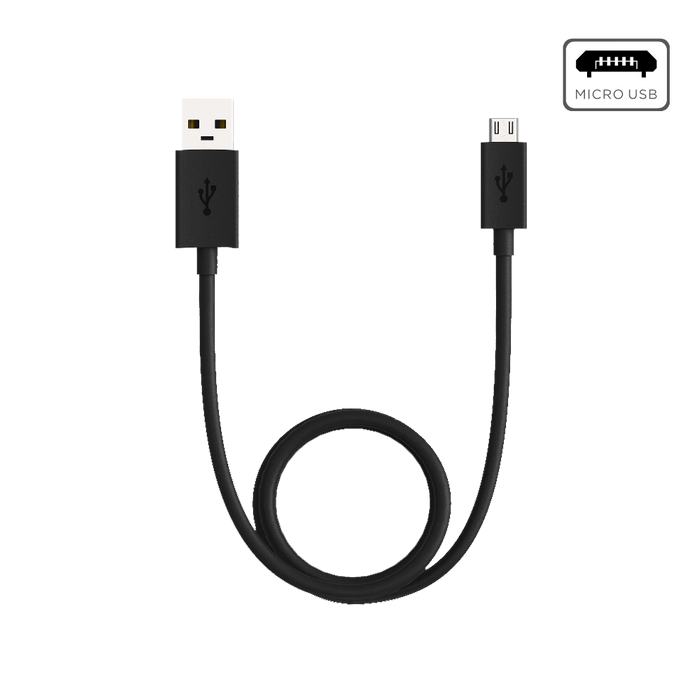
\includegraphics[scale=0.4]{Figuras/25.carregador-image-usb.png}
  \caption{Cabo MicroUSB}
  \label{fig:Cabo MicroUSB}
\end{figure}

    
\end{itemize}